%*************************************************
% In this file the first few pages are typeset.
% Make the changes accordingly
%*************************************************

% شماره صفحات با حروف
\pagenumbering{adadi}

%***************************
% 1st page: Blank
%***************************
\thispagestyle{empty}
\mbox{}
\pagebreak

%***************************
% 2nd page: Besmelah
%***************************
\thispagestyle{empty}
\begin{center}
	~\vfill
	
\includegraphics[scale=1]{besm.jpg}
	~\vfill
\end{center}
\pagebreak

%***************************
% 3rd page: Title
%***************************
\thispagestyle{empty}
%\pagenumbering{gobble}
\newgeometry{left=3cm,right=3cm,top=2cm}
\begin{center}
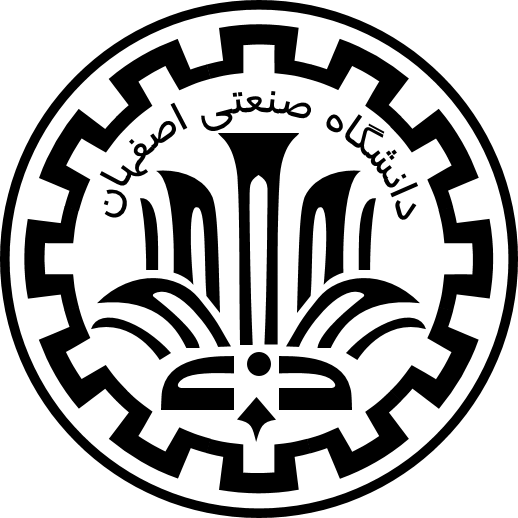
\includegraphics[height=3cm]{iut_logo.png}
\vspace{0.4cm}

\textbf{دانشگاه صنعتی اصفهان}\\
\vspace{0.4cm}

{\large

	دانشکده مهندسی برق و کامپیوتر
}
\vspace{3.5cm}

{\LARGE
	\textbf{
	بهبود کارایی الگوریتم یادگیری فدرال برای داده‌های غیرمستقل و غیریکنواخت با در نظر گرفتن میزان شباهت بین شبکه‌های عصبی در دستگاه‌های نهایی
	}
	\\
}
\vspace{3.5cm}

{\large
	پایان‌نامه کارشناسی ارشد مهندسی کامپیوتر - هوش مصنوعی
}
\vspace{1cm}

{\Large
	\textbf{علی بزرگ‌زاد}\\
}
\vspace{2.5cm}

{\large
	استادراهنما\\
}
\vspace{0.5cm}

{\Large
	\textbf{دکتر امیر خورسندی}\\
}
\vspace{3.34cm}

\textbf{1403}

\end{center}
\restoregeometry
\pagebreak

%***************************
% 4th page: Signatures
%***************************
\thispagestyle{empty}
\newgeometry{left=3cm,right=3cm,top=2cm}
\begin{center}
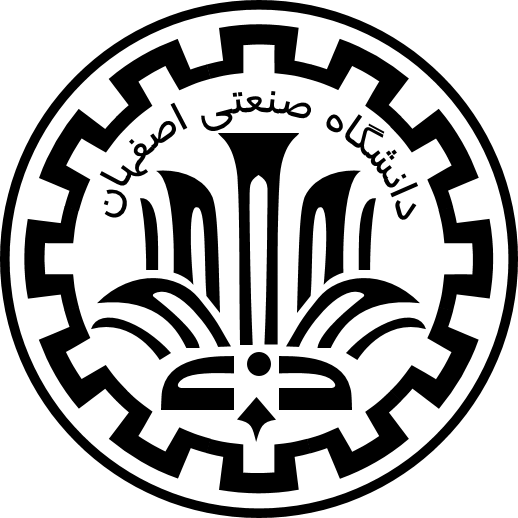
\includegraphics[height=3cm]{iut_logo.png}
\vspace{0.4cm}

\textbf{دانشگاه صنعتی اصفهان}\\
\vspace{0.4cm}

{\large
	دانشکده مهندسی برق و کامپیوتر
}
\vspace{1.8cm}

\vfill

{\Large
%	\scalebox{1}{
	پایان‌نامه کارشناسی ارشد مهندسی کامپیوتر --
	هوش مصنوعی ‎\\
	\vspace{.2cm}
	آقای علی بزرگ‌زاد
%	}
	\\
	\vspace{.3cm}
	تحت عنوان\\
}


\end{center}
\vfill
\vspace{2.5cm}

{\large
	\noindent
	\textbf{
	بهبود کارایی الگوریتم یادگیری فدرال برای داده‌های غیرمستقل و غیریکنواخت با در نظر گرفتن میزان شباهت بین شبکه‌های عصبی در دستگاه‌های نهایی
	}
}

\vspace*{2cm}

در تاریخ 1403/06/00 توسط کمیته تخصصی زیر مورد بررسی و تصویب نهایی قرار گرفت:\\
\vspace{0.8cm}

{\normalsize
	
	\begin{tabular}{rr}
	\vspace*{.8cm}
	1- استاد راهنمای پایان‌نامه  & \hspace{2cm} دکتر امیر خورسندی \\
	\vspace{.8cm}
%	2- استاد مشاور پایان‌نامه  &\hspace{2cm} دکتر پوریا پرنیانی \\
%	\vspace{.8cm}
%	3-استاد داور &\hspace{2cm} ... \\
%	\vspace{.8cm}
%	۴-استاد داور &\hspace{2cm} ... \\
%	\vspace{.8cm}
	سرپرست تحصیلات تکمیلی دانشکده &\hspace{2cm} دکتر بهزاد نظری \\
	\end{tabular}
}
\restoregeometry
\pagebreak

%***************************
% 5th page: Acknowledgment
%***************************
\thispagestyle{empty}
\newgeometry{left=3cm,right=4cm,top=4cm}
\vspace*{1.5cm}

{\large
	\textbf{تشکر و قدردانی}\\

	سپاسگزار پروردگار بزرگ هستم که در به پایان رساندن این مرحله از تحصیل مرا یاری نمود. اکنون بر خود لازم می‌دانم تا با تمام وجود از همه کسانی که در این مسیر همراه من بودند، قدردانی کنم.  
	
	از استاد راهنمای گرانقدرم، جناب آقای دکتر امیر خورسندی، که حضورشان همواره انگیزه‌بخش و قوت قلبی برای من بوده است، صمیمانه تشکر می‌کنم. بدون شک، این پایان‌نامه بدون راهنمایی‌ها و کمک‌های بی‌دریغ ایشان ممکن نمی‌شد.
	
	در نهایت، از پدر و مادر عزیزم که همواره با محبت‌های بی‌پایانشان پشتیبان من بوده‌اند، نهایت سپاس را دارم.

}
\restoregeometry
\pagebreak

%***************************
% 6th page: Rights
%***************************
\thispagestyle{empty}
\newgeometry{left=6cm,right=6cm}

\begin{spacing}{3}
\leavevmode
\vfill
\parbox{8 cm}{

\textbf{\Large
	 کلیه حقوق مالکیت مادی و معنوی مربوط به اين پايان نامه متعلق به دانشگاه صنعتی اصفهان و پدیدآورندگان است. این حقوق توسط دانشگاه صنعتي اصفهان و بر اساس خط مشی مالکیت فکری این دانشگاه، ارزش‌گذاری و سهم بندي خواهد شد.
	 هر گونه بهره برداري از محتوا، نتايج یا اقدام براي تجاري‌سازي دستاوردهاي اين پايان نامه تنها با مجوز کتبی دانشگاه صنعتی اصفهان امکان‌پذیر است.
	 }

}
\vfill
\end{spacing}
\restoregeometry
\pagebreak

%***************************
% 7th page: Dedication
%***************************
\thispagestyle{empty}
\vspace*{4cm}

{\LARGE
\centering
\textbf{تقدیم به \\ پدر و مادر عزیزم }

}
\pagebreak

%***************************
% 8th page: Table of contents
%***************************

\titleformat{\chapter}[display]
	{\normalfont\LARGE\bfseries\centering}{\chaptertitlename ~ \tartibi{chapter}}{20pt}{\LARGE}
\newgeometry{left=2.5cm,right=3cm,top=3cm,bottom=2.5cm,includehead=false,headsep=1cm,footnotesep=.5cm}
\baselineskip=.7cm

\addtocontents{toc}{\textbf{\underline{عنوان}}}
\addtocontents{toc}{\hfill\textbf{\underline{صفحه}}\par}
\addcontentsline{toc}{section}{فهرست مطالب}
\tableofcontents
\pagebreak

\addcontentsline{toc}{section}{فهرست تصاویر}
\listoffigures
\pagebreak

%\addcontentsline{toc}{section}{فهرست جداول}
%\listoftables
%\pagebreak

% change the font and margins of a chapter title
\titlespacing*{\chapter}{0pt}{3.5cm}{6cm}
\titleformat{\chapter}[display]
	{\normalfont\LARGE\bfseries\raggedright}{\chaptertitlename ~ \tartibi{chapter}}{20pt}{\LARGE}

% No page numbers on the first page of a chapter
\assignpagestyle{\chapter}{empty}
